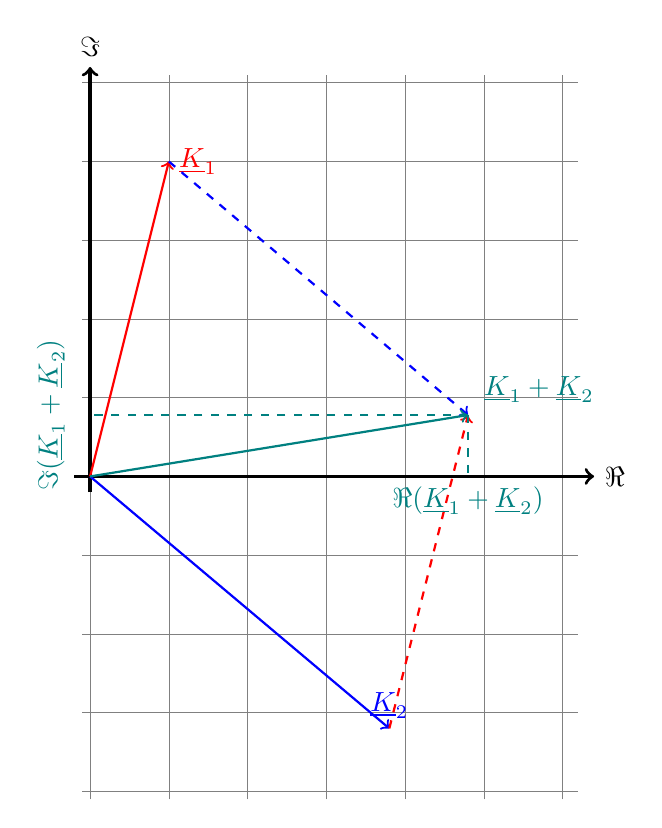
\begin{tikzpicture}
    \draw (0,0) coordinate (K);
    \draw[very thin,gray] (-0.1,-4.1) grid (6.2,5.1);
    \draw[->, very thick] (-0.2,0) -- (6.4,0) node[right] {$\Re$};
    \draw[->, very thick] (0,-0.2) -- (0,5.2) node[above] {$\Im$};
    \draw[->, thick, red] (0,0) -- (1,4) node[right] {$\underline{K}_\mathrm{1}$};
    \draw[->, thick, blue] (0,0) -- (3.8,-3.2) node[above] {$\underline{K}_\mathrm{2}$};

    \draw[->, dashed, thick, blue] (1,4) -- (4.8,0.78);
    \draw[->, dashed, thick, red] (3.8,-3.2) -- (4.8,0.78);


    \draw[->, thick, teal] (0,0) -- (4.8,0.78);
    \draw(5.7,1.1) node [teal] {$\underline{K}_\mathrm{1}+\underline{K}_\mathrm{2}$};
    \draw[dashed, thick, teal] (4.8,0.78) -- (0,0.78)
    (-0.5,0.78) node[rotate=90] {$\Im(\underline{K}_\mathrm{1}+\underline{K}_\mathrm{2}$)};
    \draw[dashed, thick, teal] (4.8,0.78) -- (4.8,0) node[below] {$\Re(\underline{K}_\mathrm{1}+\underline{K}_\mathrm{2}$)};
\end{tikzpicture}